%% LyX 2.2.3 created this file.  For more info, see http://www.lyx.org/.
%% Do not edit unless you really know what you are doing.
\documentclass[spanish]{article}
\usepackage[T1]{fontenc}
\usepackage[utf8]{luainputenc}
\usepackage{geometry}
\geometry{verbose,tmargin=2cm,bmargin=2cm,lmargin=2cm,rmargin=2cm,headheight=2cm,headsep=2cm}
\setlength{\parindent}{0bp}
\usepackage{float}
\usepackage{graphicx}
\usepackage{babel}
\addto\shorthandsspanish{\spanishdeactivate{~<>}}

\begin{document}

\section{Circuito no inversor}

A lo largo de esta seccion se procedera a analizar el comportamiento
ideal y real del amplificador operacional \emph{LM324 }conectado como
se muestra en la figura \ref{1_b_1}. Considerando los valores de
los componentes como se puede ver en la tabla \ref{1_a_t_1}. 

\begin{figure}[H]
\begin{centering}
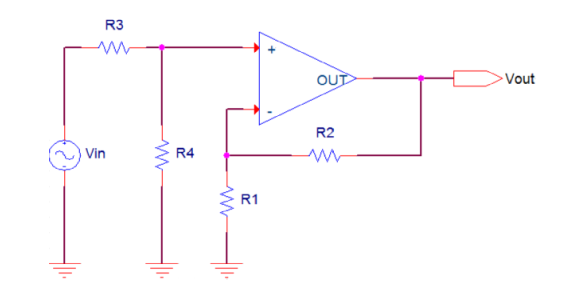
\includegraphics[scale=0.5]{Resources1b/circuit}
\par\end{centering}
\caption{Circuito B}
\label{1_b_1}

\end{figure}

\subsection{Transferencia}

Comenzando por el analisis ideal, se pidió calcular y graficar la
relación $\frac{V_{out}}{V_{in}}$, esto quiere decir, considerando
$a_{0}$ finito y $A(\omega)$ con polo dominante. Considerando las
siguientes ecuaciones descriptas a continuacion y operando correctamente,
se llega a que la relacion $\frac{V_{out}}{V_{in}}$ esta dada por
la ecuación (\ref{eq:1_b_1}).

\begin{equation}
H(s)=\frac{R_{4}\omega_{p}a_{0}\left(R_{1}+R_{2}\right)}{\left(R_{3}-R_{4}\right)\left(R_{1}\omega_{p}a_{0}+\left(R_{1}+R_{2}\right)\left(\omega_{p}+s\right)\right)}\label{eq:1_b_1}
\end{equation}

\[
H(s)=\frac{414\times10^{9}}{110\times10^{3}s+47\times10^{9}}\,\,\,Caso\,1
\]

\[
H(s)=\frac{75\times10^{9}}{20\times10^{3}s+47\times10^{9}}\,\,\,Caso\,2
\]

\[
H(s)=\frac{414\times10^{9}}{110\times10^{3}s+471\times10^{9}}\,\,\,Caso\,3
\]

\begin{figure}[H]
\begin{centering}
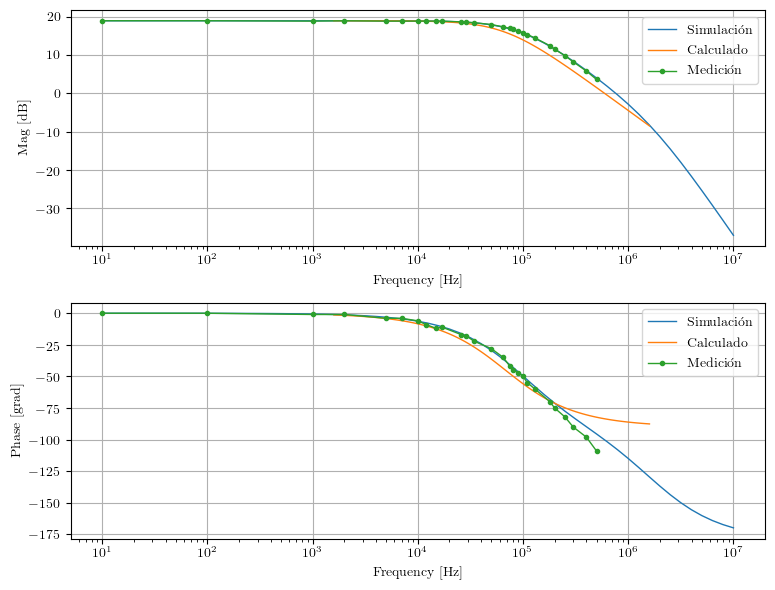
\includegraphics[scale=0.5]{Resources1b/H1b}
\par\end{centering}
\caption{Comportamiento del circuito para el caso 1}
\end{figure}

\begin{figure}[H]
\begin{centering}
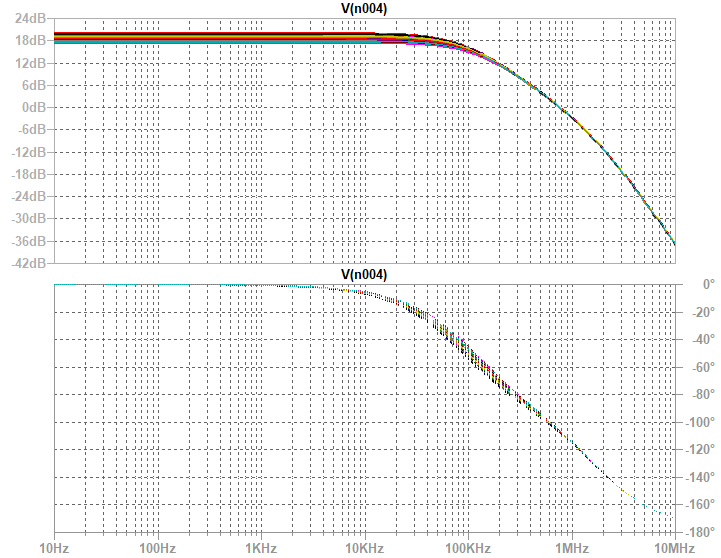
\includegraphics[scale=0.5]{Resources1b/Montecarlo1}
\par\end{centering}
\caption{Análisis montecarlo del caso 1}
\end{figure}

\begin{figure}[H]
\begin{centering}
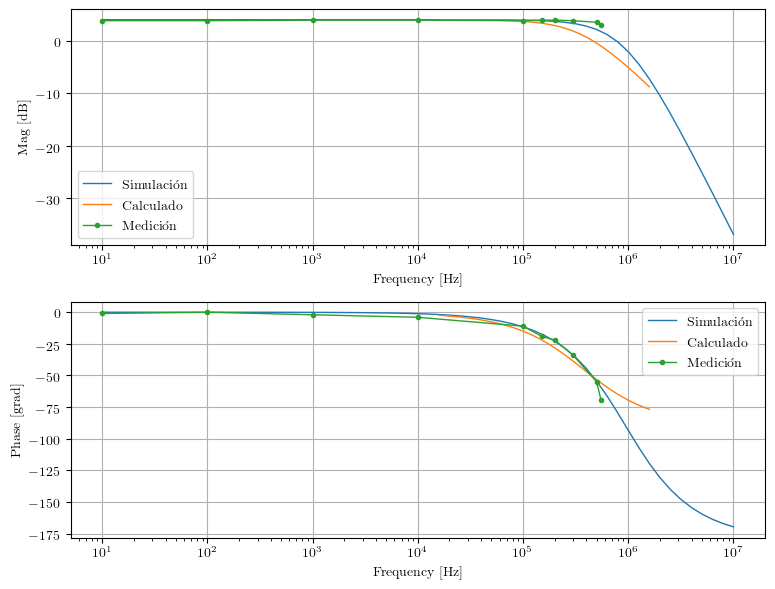
\includegraphics[scale=0.5]{Resources1b/H2b}
\par\end{centering}
\caption{Comportamiento del circuito para el caso 2}
\end{figure}

\begin{figure}[H]
\begin{centering}
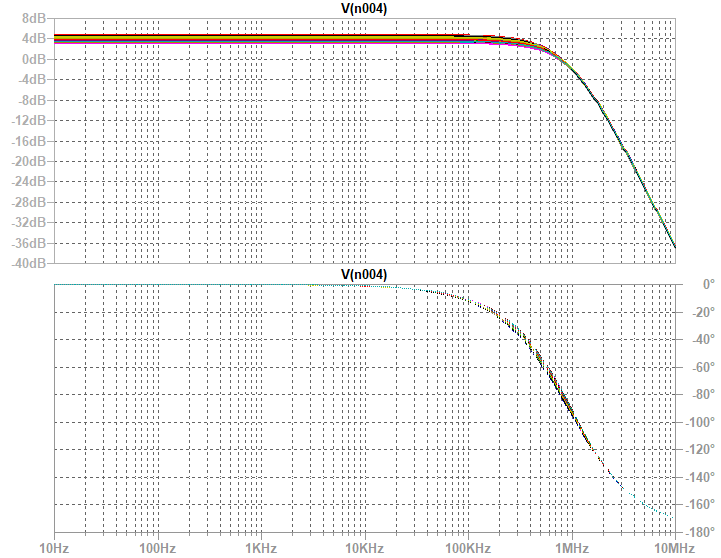
\includegraphics[scale=0.5]{Resources1b/Montecarlo2}
\par\end{centering}
\caption{Análisis montecarlo del caso 2}
\end{figure}

\begin{figure}[H]
\begin{centering}
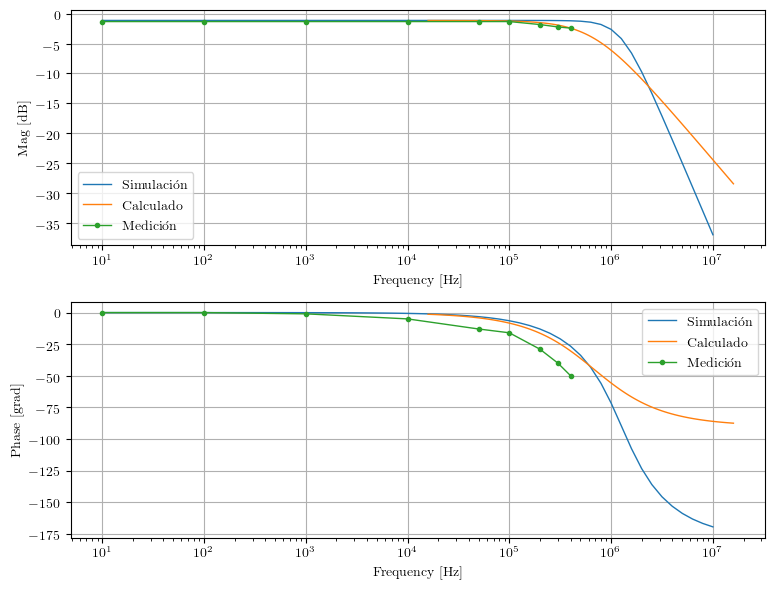
\includegraphics[scale=0.5]{Resources1b/H3b}
\par\end{centering}
\caption{Comportamiento del circuito para el caso 3}
\end{figure}

\begin{figure}[H]
\begin{centering}
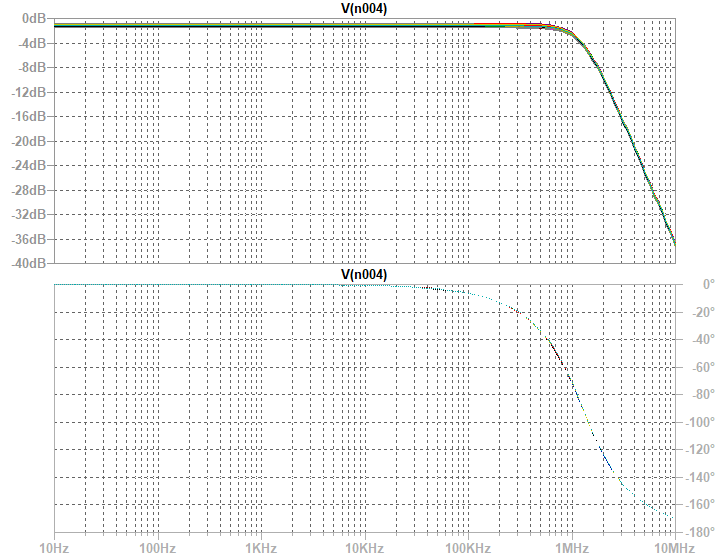
\includegraphics[scale=0.5]{Resources1b/Montecarlo3}
\par\end{centering}
\caption{Análisis montecarlo del caso 3}
\end{figure}

\subsection{Impedancia de entrada}

Consecuentemente, se nos instó a calcular la impedancia de entrada
vista por el generador hacia nuestro circuito. Nuevamente, se utilizo
el \emph{Circuit Solver }creado en Python para calcular las expresiones
de las impedancias de entrada. La ecuacion que describe la impedancia
de entrada se detalla en la ecuación (\ref{eq:1_b_2}).

\begin{equation}
Z_{inp}=R_{3}+R_{4}\label{eq:1_b_2}
\end{equation}

Por lo tanto, las impedancias de entrada para cada caso serán;

\[
Z_{inp}=50(k\Omega)\,\,\,Caso\,1
\]

\[
Z_{inp}=50(k\Omega)\,\,\,Caso\,2
\]

\[
Z_{inp}=500(k\Omega)\,\,\,Caso\,3
\]

Teniendo en cuenta estos resultado, y a diferencia de lo visto previamente
en el análisis del circuito inversor, se puede observar como la impedancia
de entrada permanece constante frente a cambios de frecuencia en la
tension de entrada.

\subsection{Alinialidades}

\subsubsection{Saturacion}

\[
V_{in}\leq\frac{Vcc\left(R_{3}+R_{4}\right)\sqrt{4\pi^{2}f^{2}\left(R_{1}+R_{2}\right)^{2}+\left(R_{1}Wa_{0}+R_{1}W+R_{2}W\right)^{2}}}{R_{4}Wa_{0}\left(R_{1}+R_{2}\right)}
\]

\[
V_{in}\leq2.41112589934996\cdot10^{-12}Vcc\sqrt{48400000000\pi^{2}f^{2}+2.22172559899497\cdot10^{21}}\,\,\,Caso\,1
\]

\[
V_{in}\leq1.32611924464248\cdot10^{-11}Vcc\sqrt{1600000000\pi^{2}f^{2}+2.22132575036449\cdot10^{21}}\,\,\,Caso\,2
\]

\[
V_{in}\leq2.41112589934996\cdot10^{-12}Vcc\sqrt{48400000000\pi^{2}f^{2}+2.22128576748057\cdot10^{23}}\,\,\,Caso\,3
\]

\begin{figure}[H]
\begin{centering}
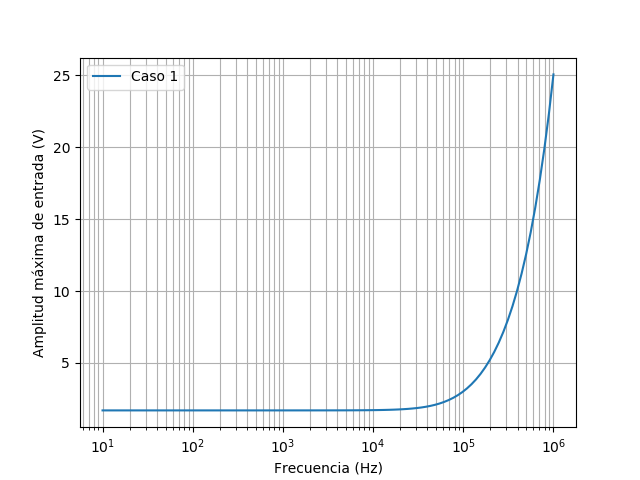
\includegraphics[scale=0.5]{Resources1b/sat1}
\par\end{centering}
\caption{Tension de entrada máxima respecto de la frecuencia de entrada para
que no ocurra saturación en el caso 1}

\end{figure}

\begin{figure}[H]
\begin{centering}
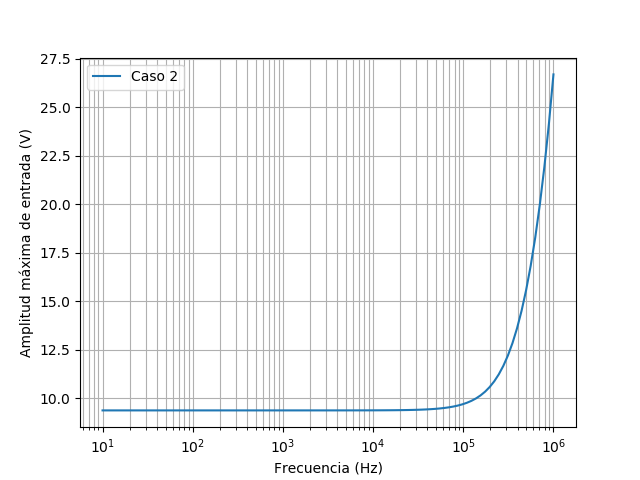
\includegraphics[scale=0.5]{Resources1b/sat2}
\par\end{centering}
\caption{Tension de entrada máxima respecto de la frecuencia de entrada para
que no ocurra saturación en el caso 2}
\end{figure}

\begin{figure}[H]
\begin{centering}
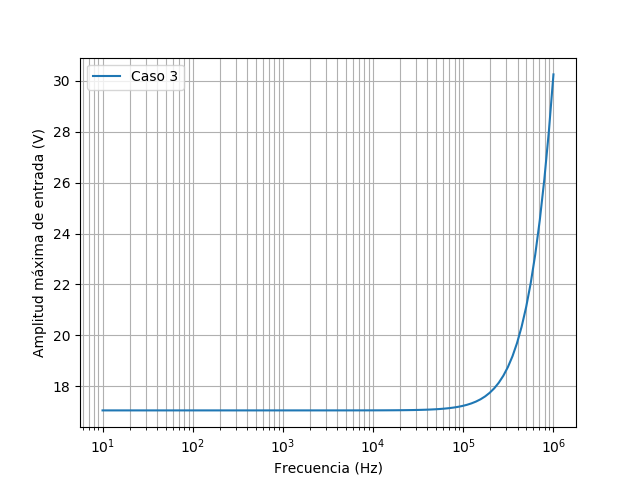
\includegraphics[scale=0.5]{Resources1b/sat3}
\par\end{centering}
\caption{Tension de entrada máxima respecto de la frecuencia de entrada para
que no ocurra saturación en el caso 3}
\end{figure}

\begin{figure}[H]
\begin{centering}
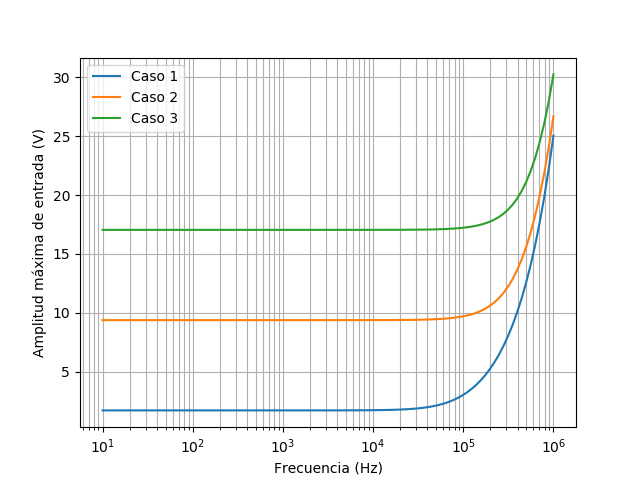
\includegraphics[scale=0.5]{Resources1b/sat123}
\par\end{centering}
\caption{Tension de entrada máxima respecto de la frecuencia de entrada para
que no ocurra saturación}
\end{figure}

\subsubsection{Slew Rate}

\[
V_{in}\leq\frac{SR\left(R_{3}+R_{4}\right)\sqrt{4\pi^{2}f^{2}\left(R_{1}+R_{2}\right)^{2}+\left(R_{1}Wa_{0}+R_{1}W+R_{2}W\right)^{2}}}{2\pi R_{4}Wa_{0}f\left(R_{1}+R_{2}\right)}
\]

\[
V_{in}\leq\frac{1.20556294967498\cdot10^{-12}SR\sqrt{48400000000\pi^{2}f^{2}+2.22172559899497\cdot10^{21}}}{\pi f}\,\,\,Caso\,1
\]

\[
V_{in}\leq\frac{6.63059622321239\cdot10^{-12}SR\sqrt{1600000000\pi^{2}f^{2}+2.22132575036449\cdot10^{21}}}{\pi f}\,\,\,Caso\,2
\]

\[
V_{in}\leq\frac{1.20556294967498\cdot10^{-12}SR\sqrt{48400000000\pi^{2}f^{2}+2.22128576748057\cdot10^{23}}}{\pi f}\,\,\,Caso\,3
\]

\begin{figure}[H]
\begin{centering}
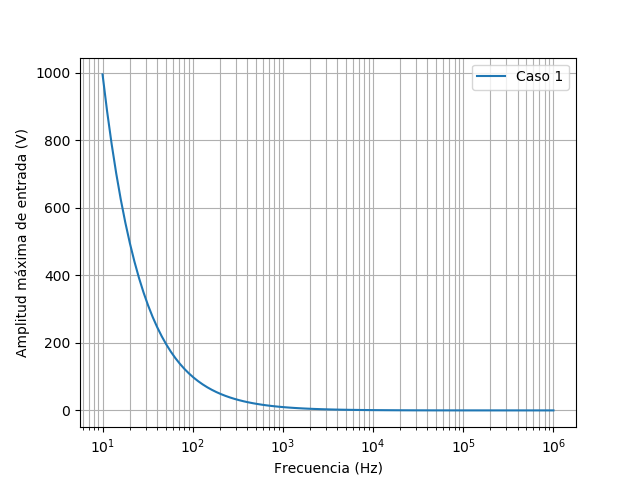
\includegraphics[scale=0.5]{Resources1b/slewRate1}
\par\end{centering}
\caption{Tension de entrada máxima respecto de la frecuencia de entrada para
que no ocurra Slew Rate en el caso 1}
\end{figure}

\begin{figure}[H]
\begin{centering}
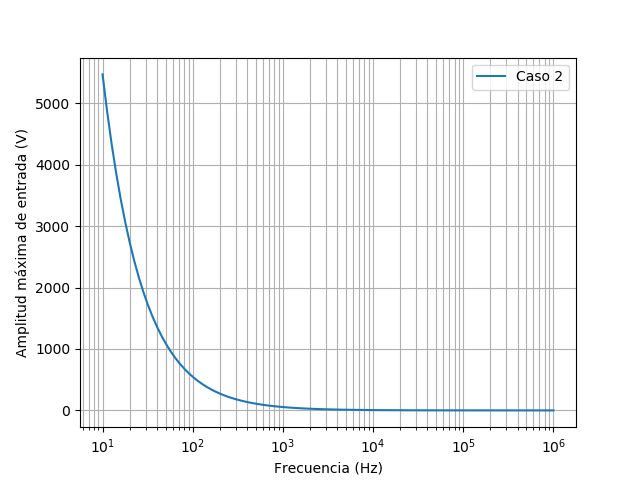
\includegraphics[scale=0.5]{Resources1b/slewRate2}
\par\end{centering}
\caption{Tension de entrada máxima respecto de la frecuencia de entrada para
que no ocurra Slew Rate en el caso 2}
\end{figure}

\begin{figure}[H]
\begin{centering}
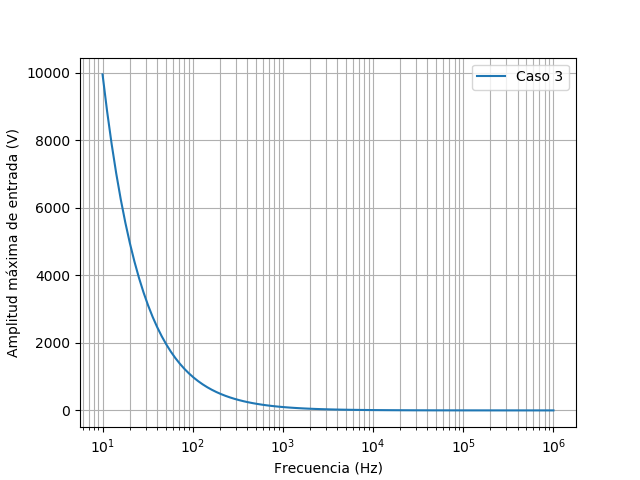
\includegraphics[scale=0.5]{Resources1b/slewRate3}
\par\end{centering}
\caption{Tension de entrada máxima respecto de la frecuencia de entrada para
que no ocurra Slew Rate en el caso 3}
\end{figure}

\begin{figure}[H]
\begin{centering}
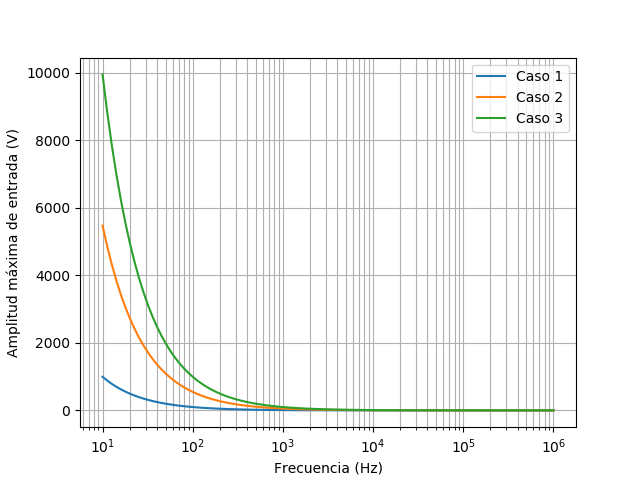
\includegraphics[scale=0.5]{Resources1b/slewRate123}
\par\end{centering}
\caption{Tension de entrada máxima respecto de la frecuencia de entrada para
que no ocurra Slew Rate}
\end{figure}

\subsubsection{Conclusiones}

\begin{figure}[H]
\begin{centering}
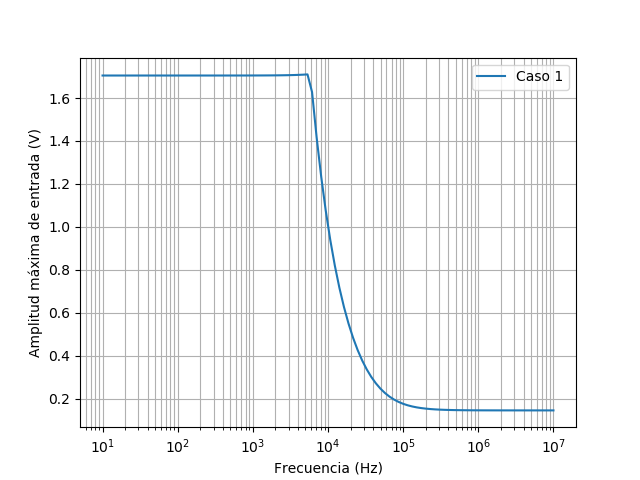
\includegraphics[scale=0.5]{Resources1b/AmplMaxVsFreq1}
\par\end{centering}
\caption{Tensión máxima de entrada para que no ocurran alinialidades en el
caso 1}

\end{figure}

\begin{figure}[H]
\begin{centering}
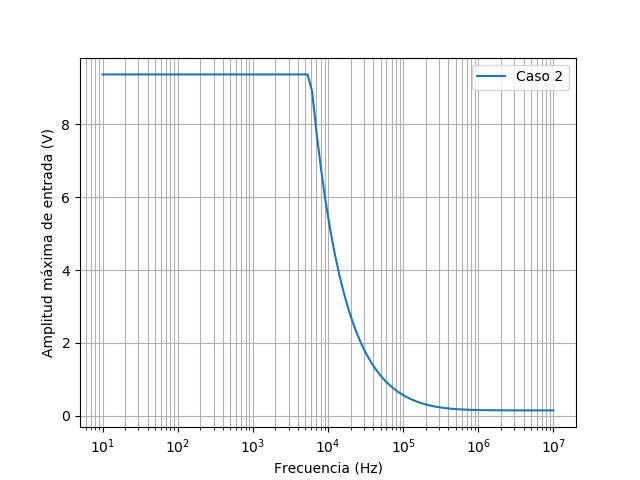
\includegraphics[scale=0.5]{Resources1b/AmplMaxVsFreq2}
\par\end{centering}
\caption{Tensión máxima de entrada para que no ocurran alinialidades en el
caso 2}
\end{figure}

\begin{figure}[H]
\begin{centering}
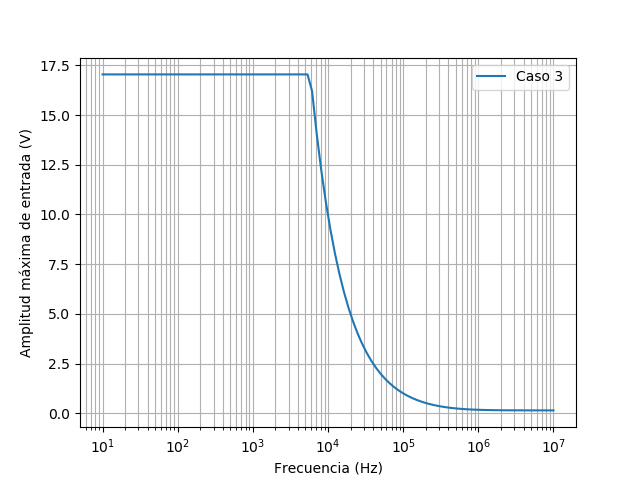
\includegraphics[scale=0.5]{Resources1b/AmplMaxVsFreq3}
\par\end{centering}
\caption{Tensión máxima de entrada para que no ocurran alinialidades en el
caso 3}
\end{figure}

\begin{figure}[H]
\begin{centering}
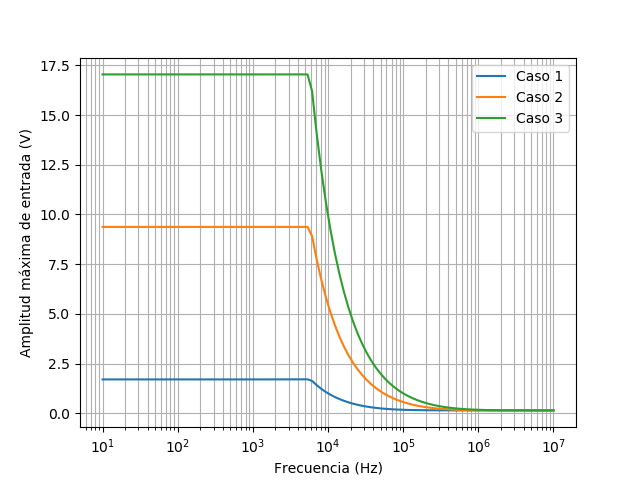
\includegraphics[scale=0.5]{Resources1b/AmplMaxVsFreq123}
\par\end{centering}
\caption{Tensión máxima de entrada para que no ocurran alinialidades}
\end{figure}

\end{document}
